\documentclass[aspectratio=169,10pt]{beamer}
\usetheme{default}
\usecolortheme{seahorse}
\setbeamertemplate{navigation symbols}{}
\setbeamertemplate{footline}[frame number]
\usepackage{graphicx, booktabs, siunitx}
\graphicspath{{../figures/}}
\title{SiPM-Wall MIP Calibration from Wall--Plastic Coincidences}
\subtitle{n\_TOF EAR2 X17 --- run 224404 (first beam data, July 15)}
\author{Dylan Neff \\[0.5ex] {\small analysis and slides prepared with Claude (Anthropic AI assistant)}}
\date{July 17, 2026}

\begin{document}

\begin{frame}\titlepage\end{frame}

\begin{frame}{Data \& selection}
\begin{itemize}
\item Official processed file, run 224404: 3792 bunches (1471 dedicated), $\sim$300M hits.
\item Per-channel ADC$\to$mV from DAQ settings ($\approx$0.0305 mV/count).
\item \alert{SiPM walls delivered no data for 46\% of beam-on bunches (643--2212)} ---
      plastics unaffected; hardware cause TBD with DAQ crew.
\item All results: post-recovery bunches, hits $>$0.1 ms after $\gamma$-flash
      (highest coincidence purity).
\end{itemize}
\end{frame}

\begin{frame}{Method: coincidences with sideband subtraction}
\centering
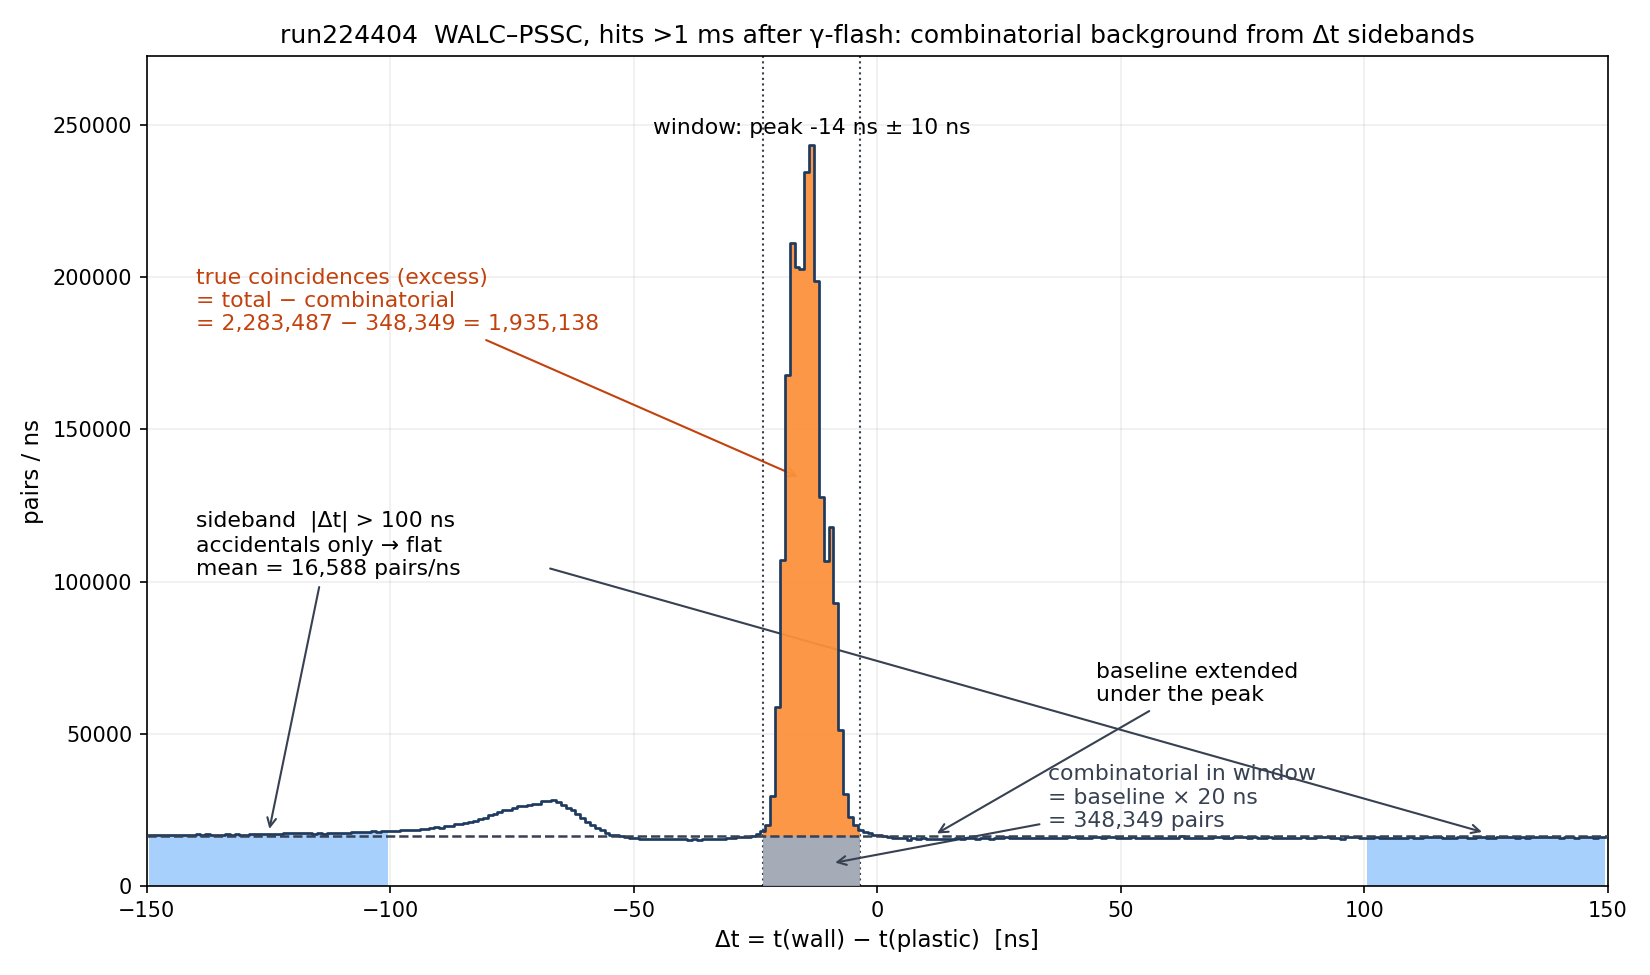
\includegraphics[height=.78\textheight]{05_sideband_diagram/sideband_method.png}
\end{frame}

\begin{frame}{What the coincidence selects}
\centering
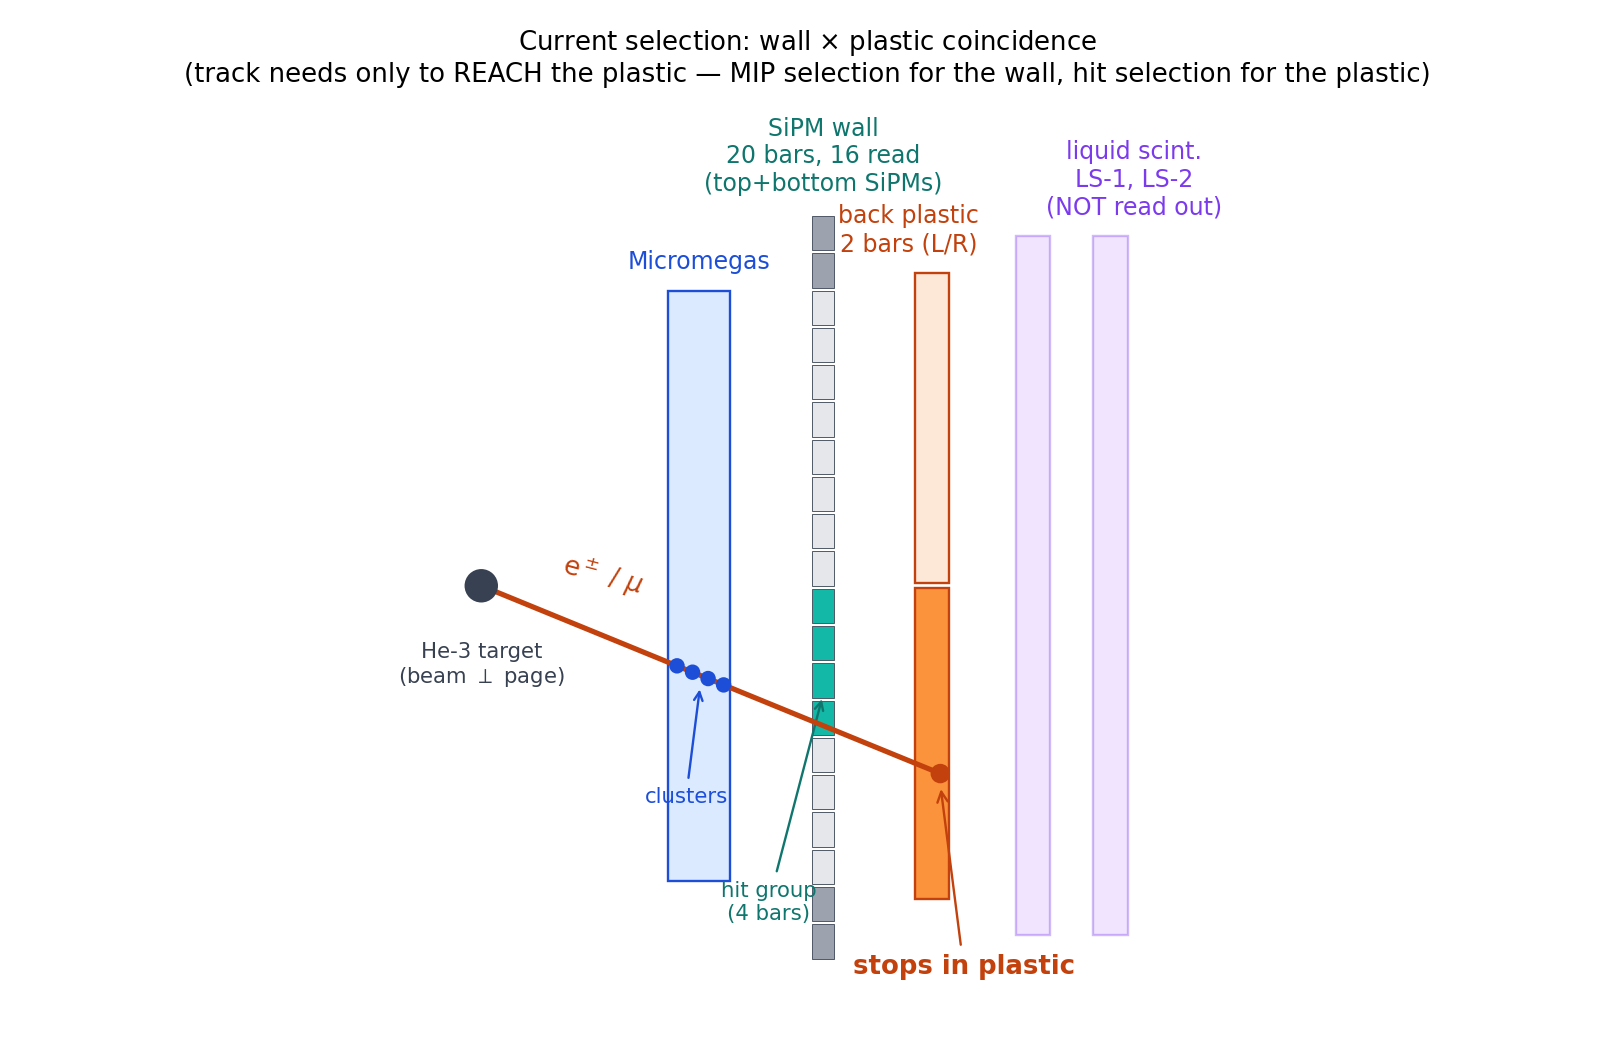
\includegraphics[height=.82\textheight]{11_diagrams/concept_wall_plastic.png}
\end{frame}

\begin{frame}{Every arm pairs wall $\leftrightarrow$ plastic cleanly}
\centering
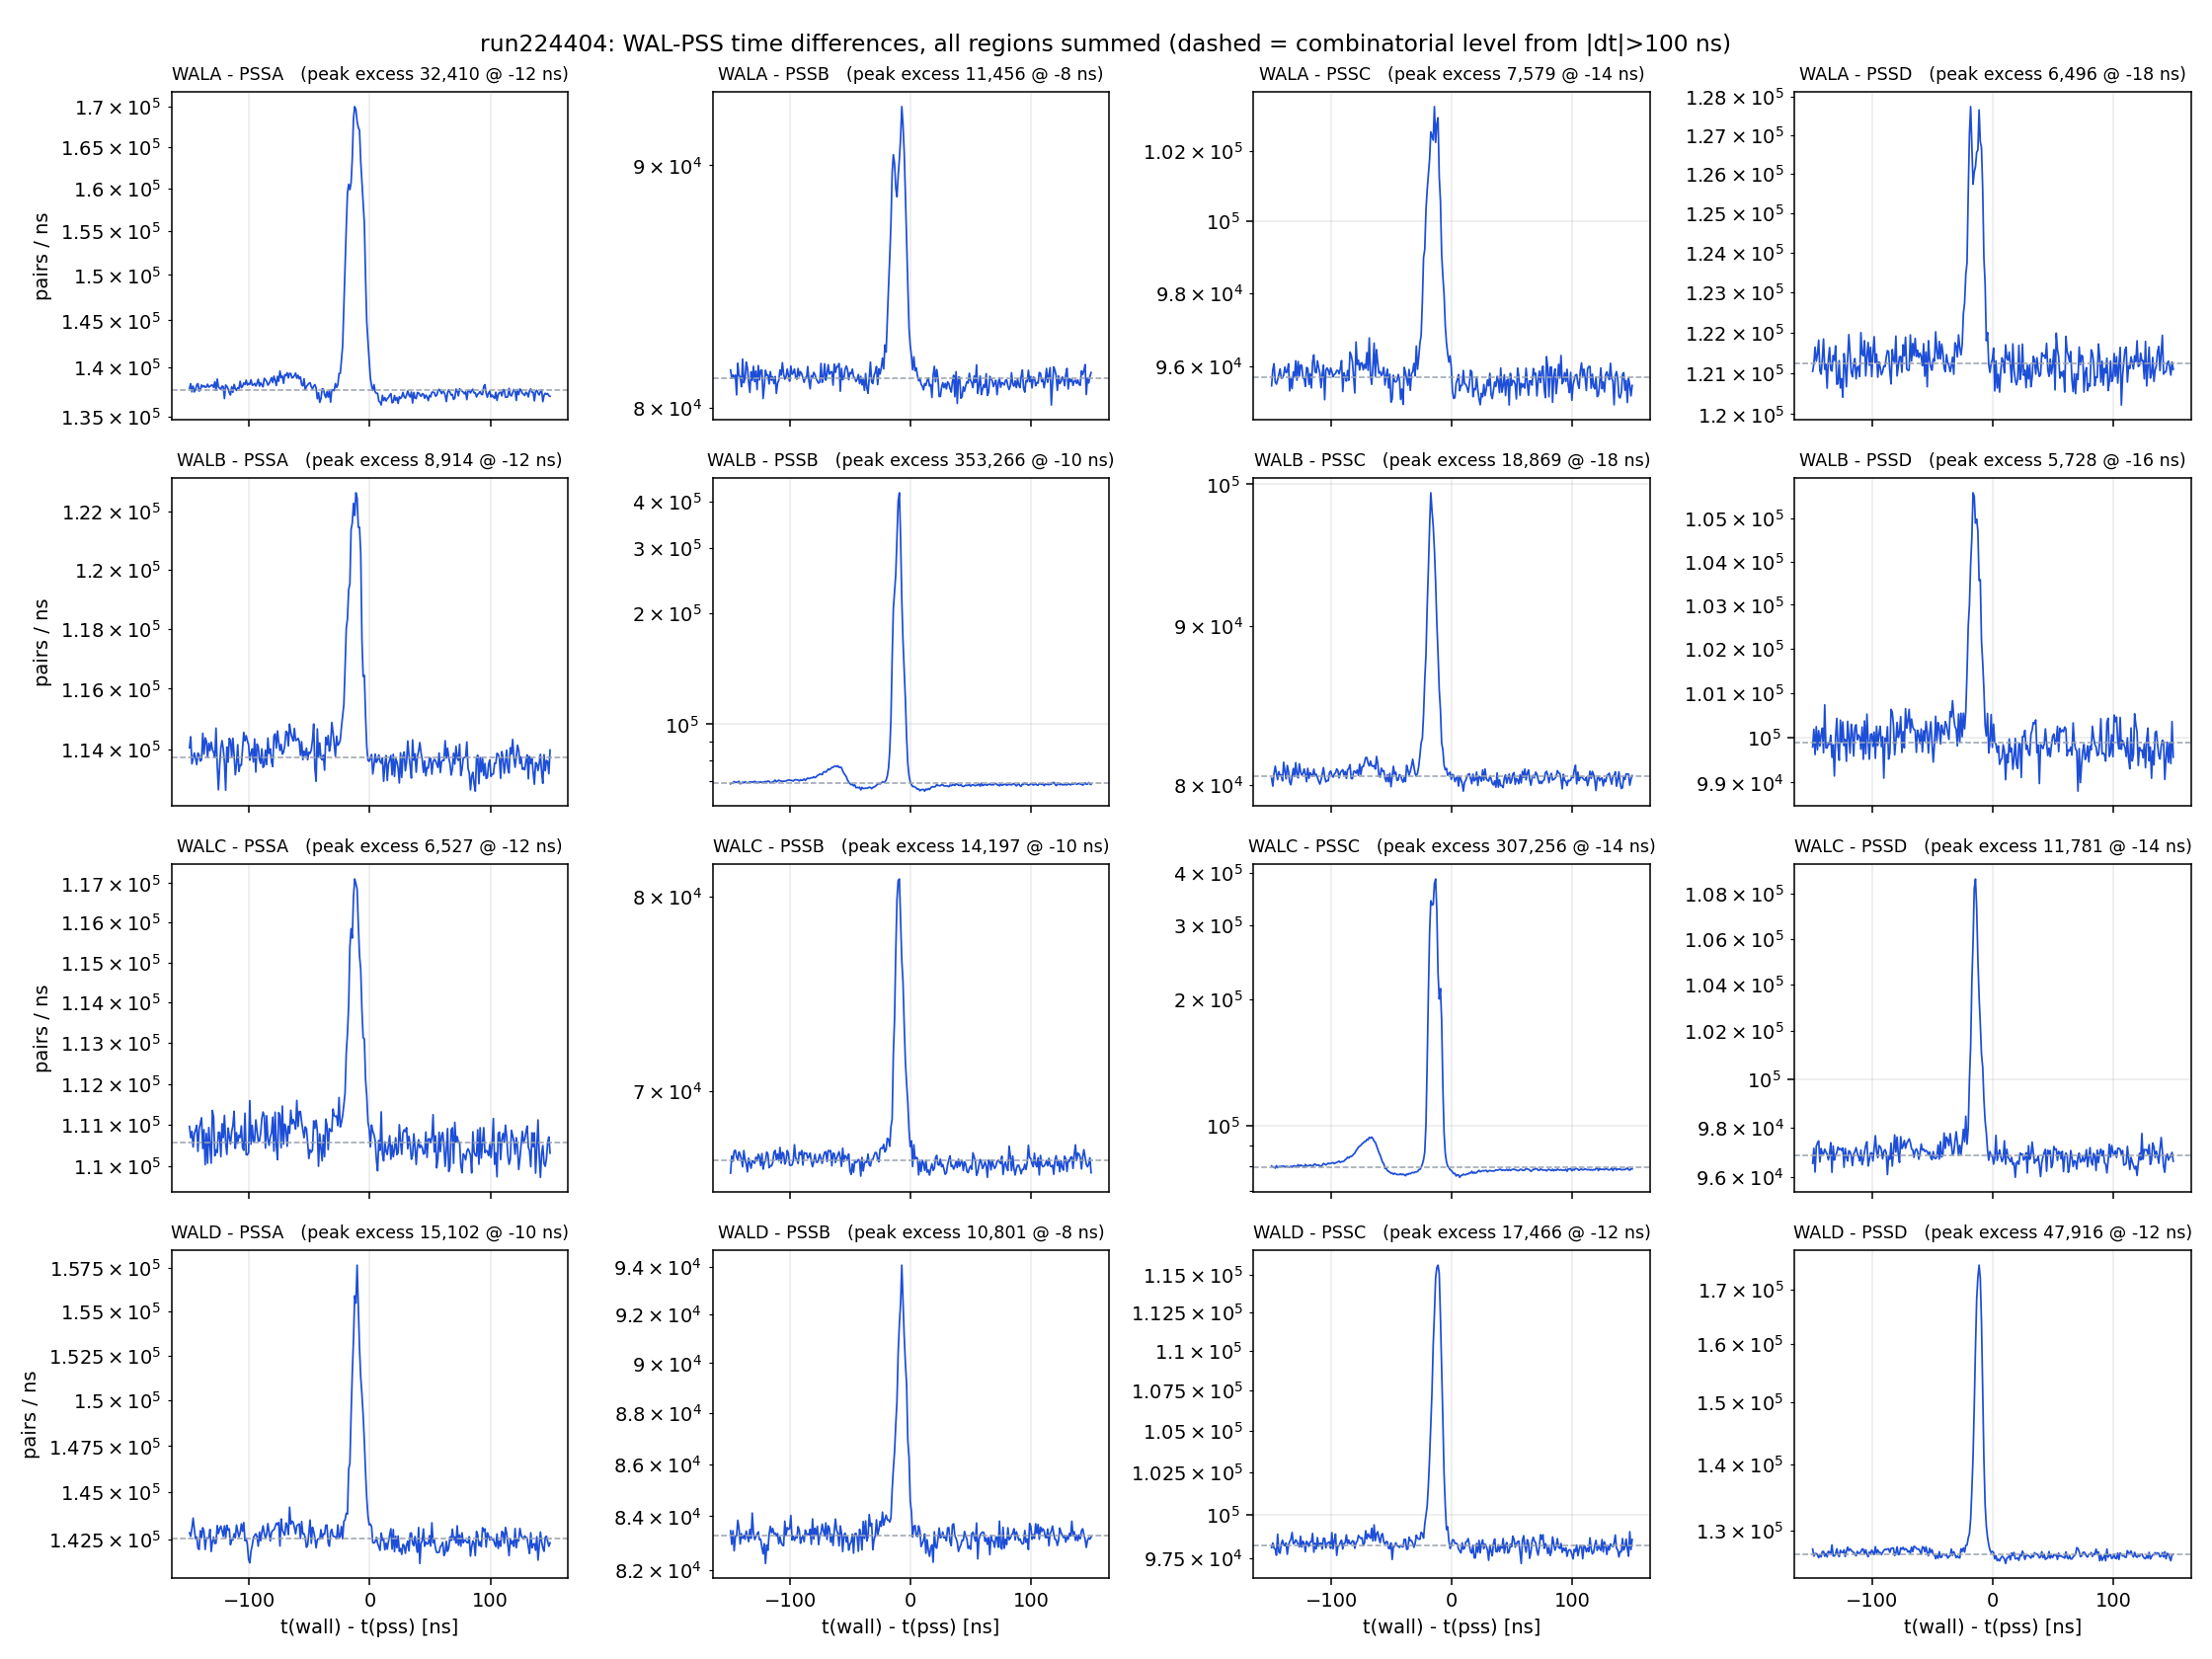
\includegraphics[height=.72\textheight]{02_coincidence/dt_matrix.png}\\
{\footnotesize Peaks at $-8$ to $-18$ ns, rms 1.5--3.5 ns; per-channel offsets
now a stored calibration.}
\end{frame}

\begin{frame}{Geometry confirmed in data}
\centering
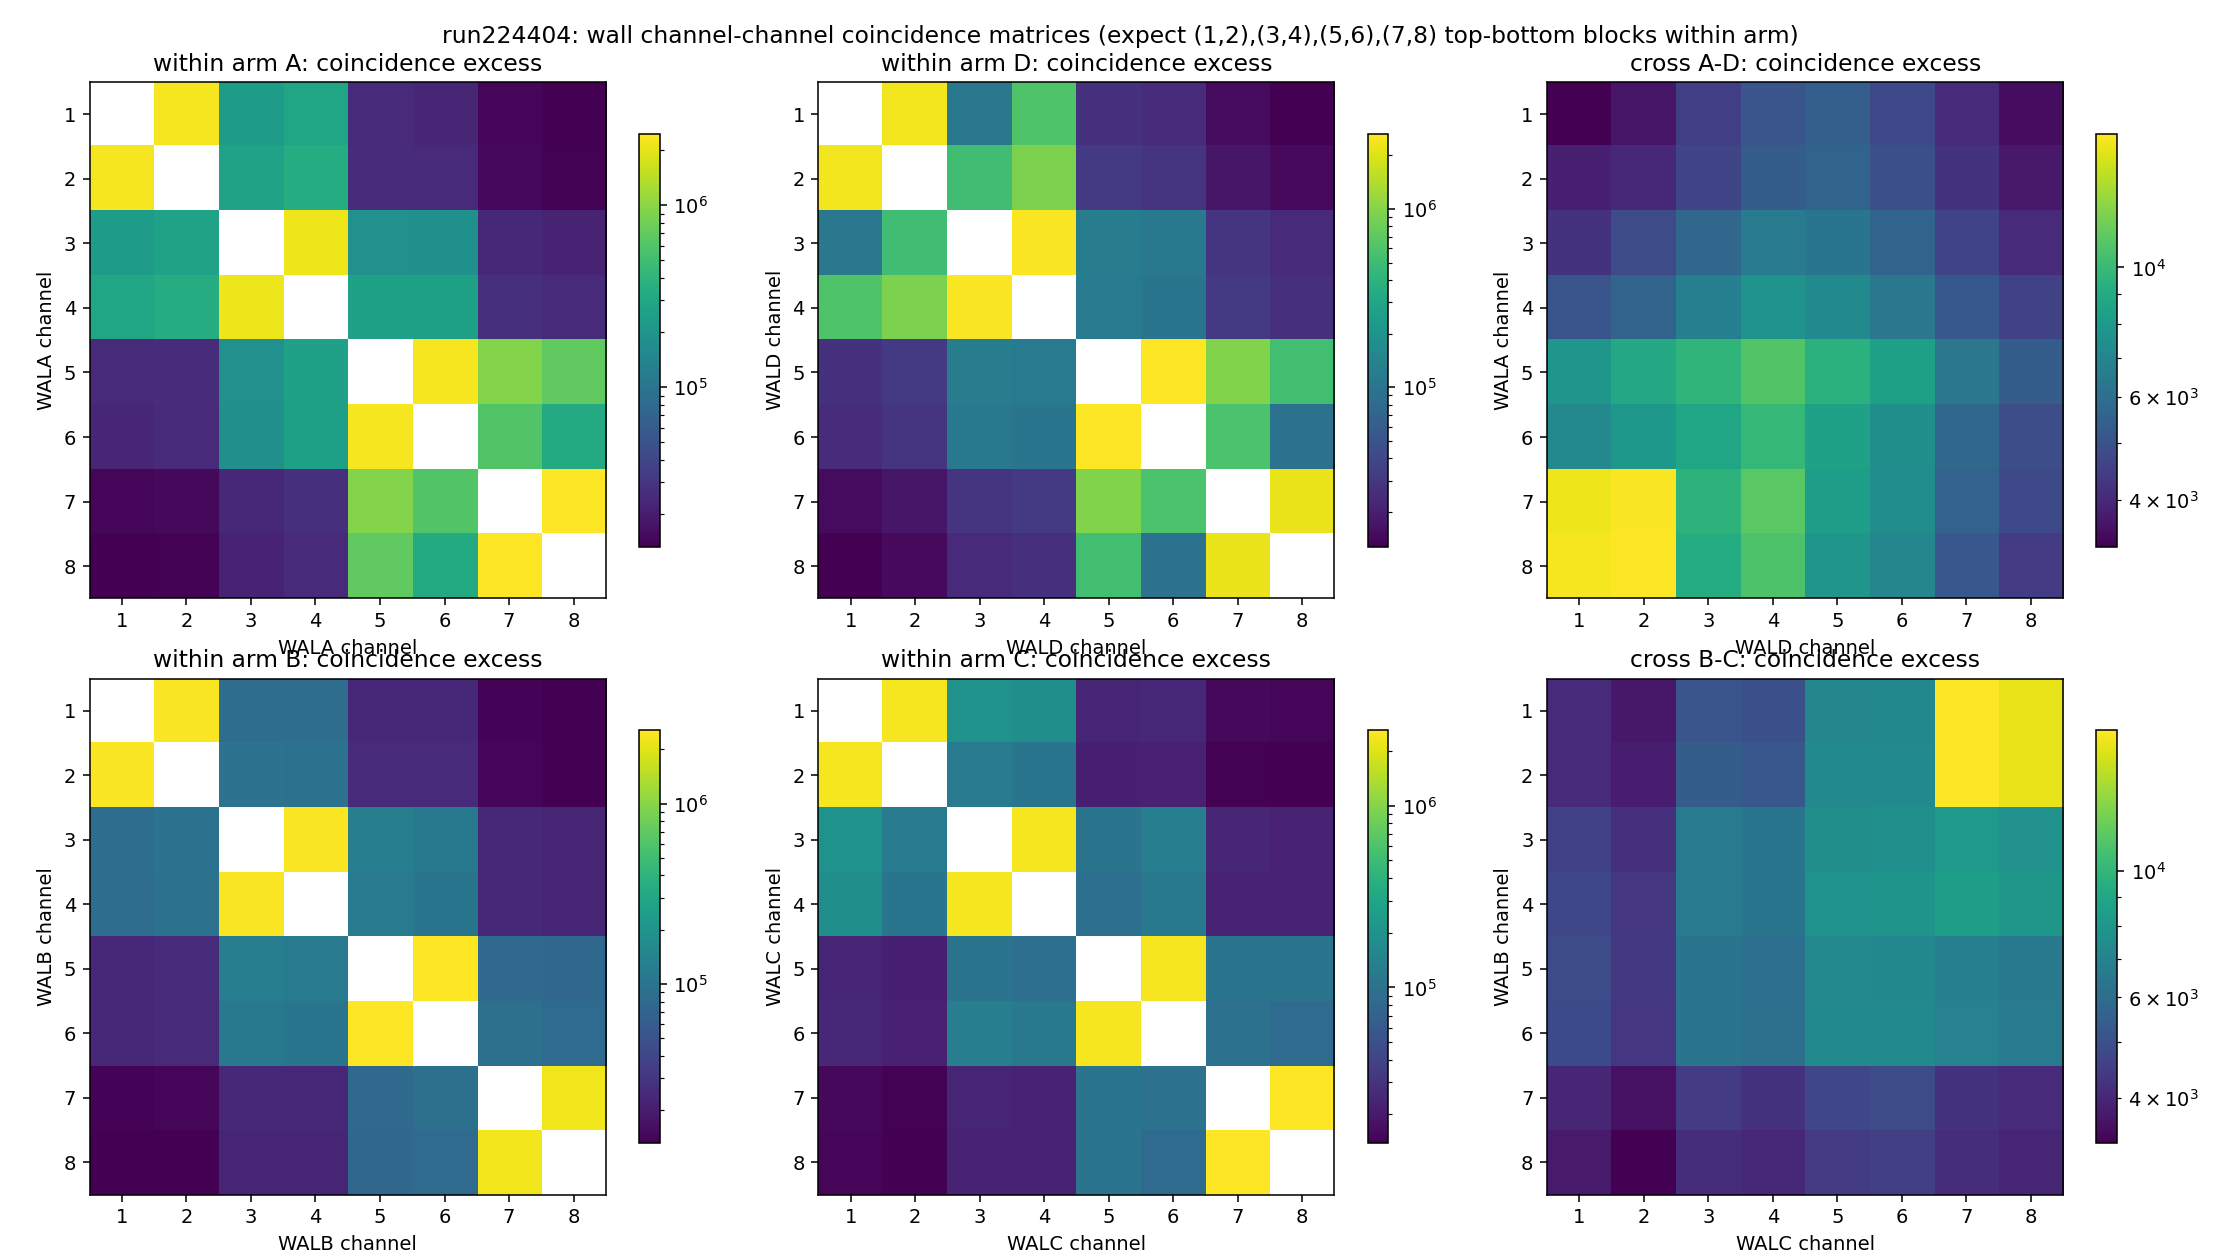
\includegraphics[height=.62\textheight]{06_07_geometry_mip/wall_geometry_matrices.png}\\
{\footnotesize Top/bottom blocks (1,2)(3,4)(5,6)(7,8) per 4-bar group; groups ordered
left$\to$right across the two bars. Corner hotspots $\Rightarrow$ A--D and B--C are
\emph{adjacent} arms. Odd=top is an assumption --- need cabling sheet.}
\end{frame}

\begin{frame}{Headline: SiPM-wall MIP peaks on arms B and C}
\centering
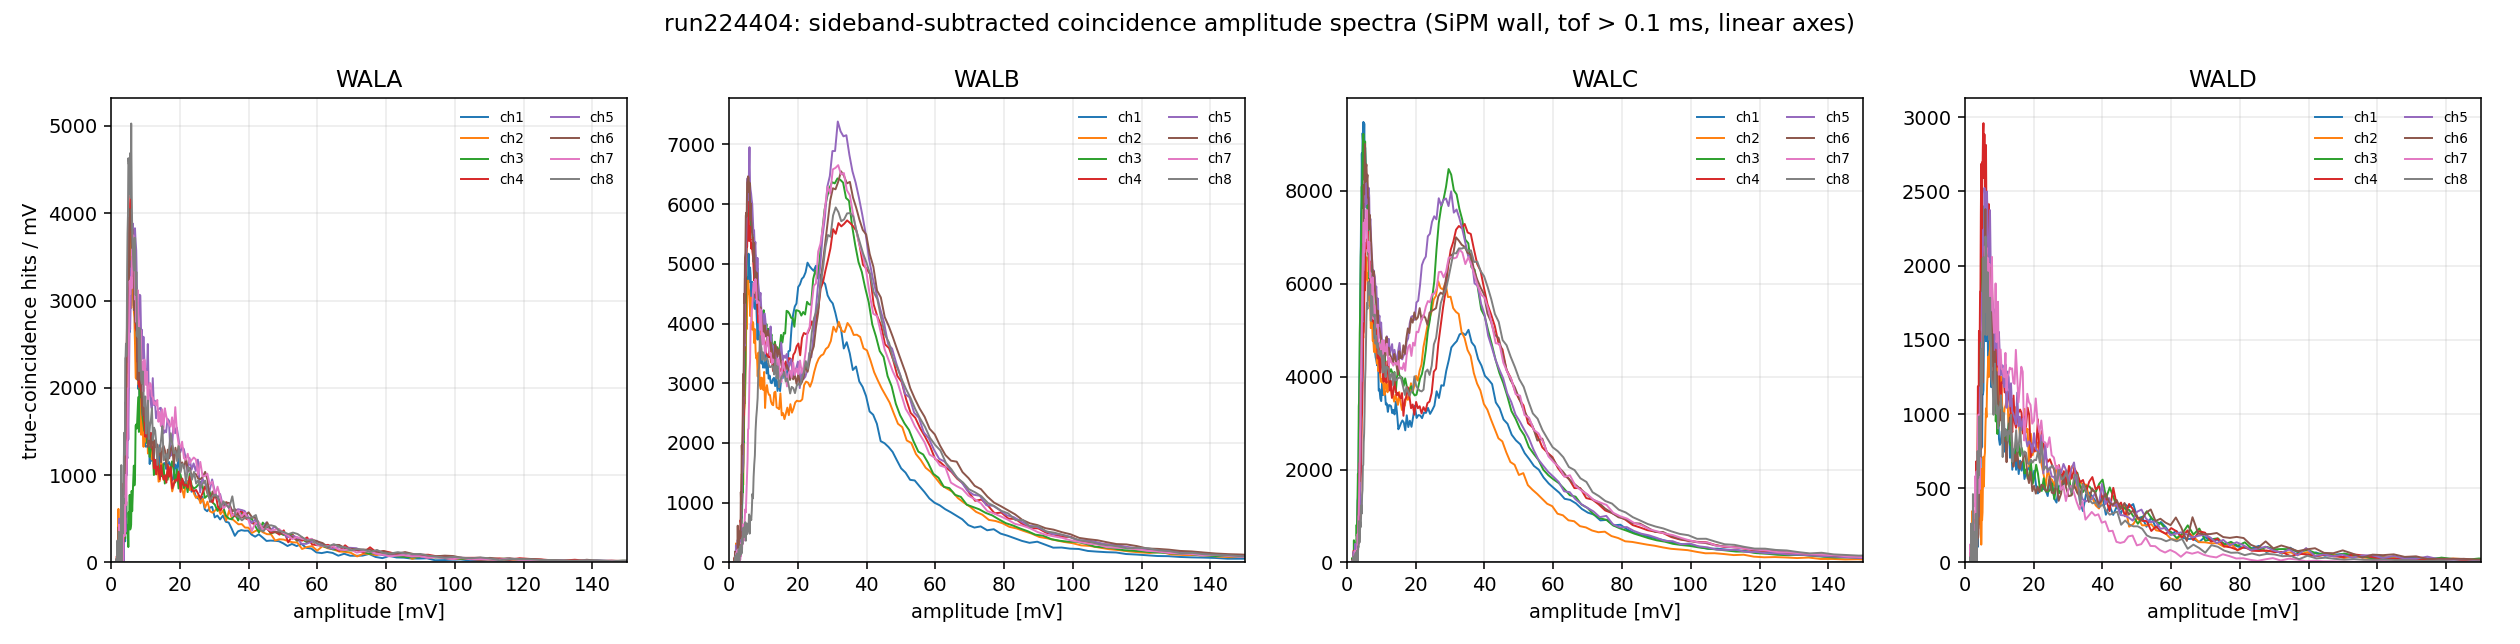
\includegraphics[width=\textwidth]{06_07_geometry_mip/mip_wall_spectra_linear.png}\\
{\footnotesize Sideband-subtracted coincidence spectra. \textbf{B/C: clean MIP
peaks, 29--39 mV, all 16 channels} $\Rightarrow$ per-channel calibration.
A/D: no MIP population (see later).}
\end{frame}

\begin{frame}{Coincidence selection performs exactly as intended (B/C)}
\centering
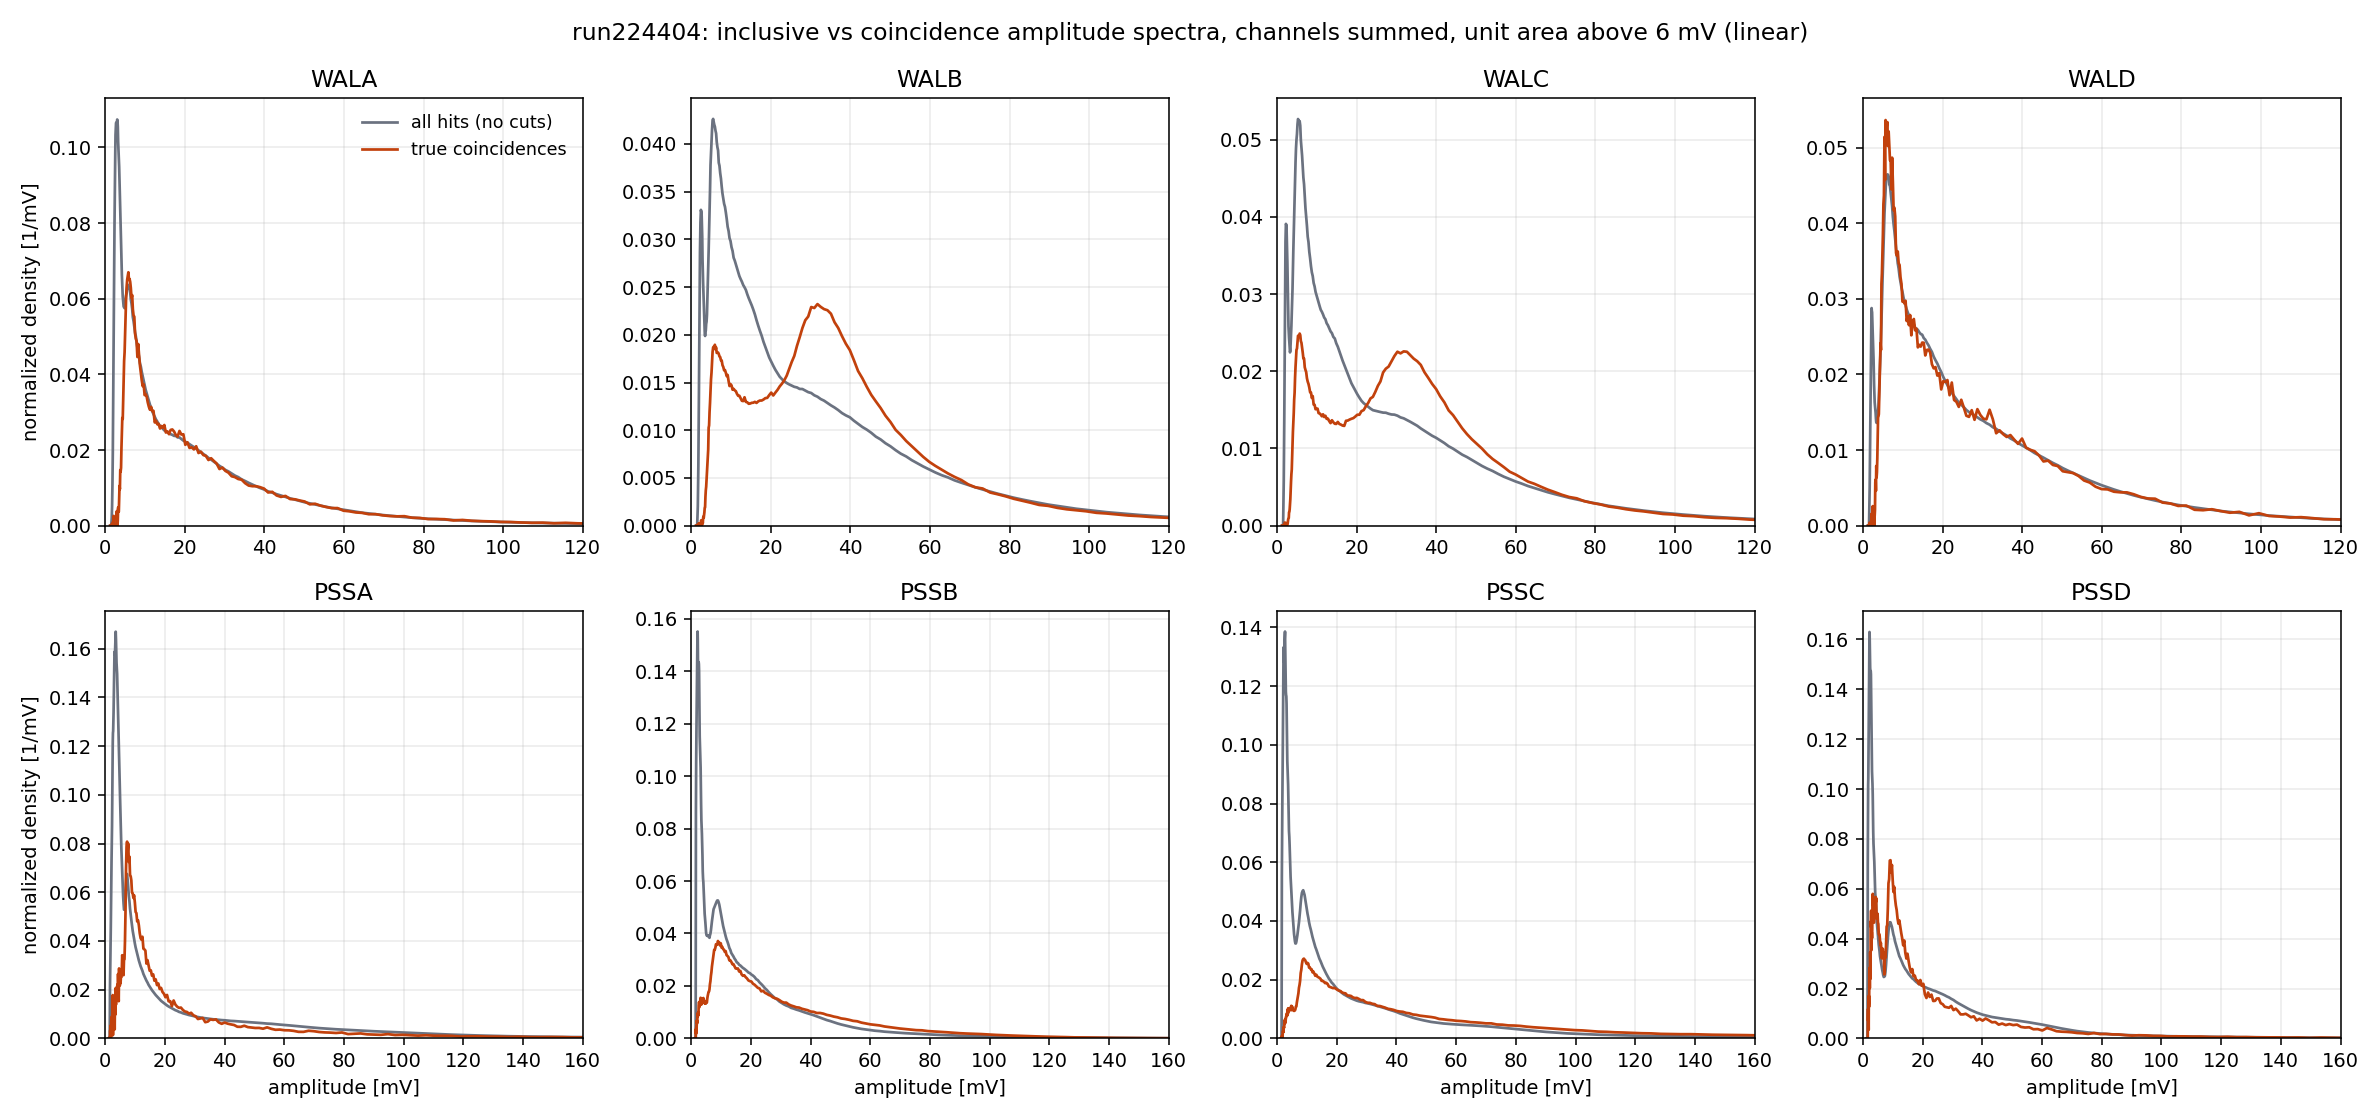
\includegraphics[width=.95\textwidth]{08_inclusive_vs_coinc/inclusive_vs_coinc_linear.png}\\
{\footnotesize Unit-normalized. Physics note: the plastic is at the \emph{back}
of the stack $\Rightarrow$ the coincidence is a through-going (MIP) selection
\emph{for the wall}, but only a hit selection for the plastic --- plastic
spectra are NOT MIP spectra.}
\end{frame}

\begin{frame}{The A/D problem --- cause still open}
\begin{columns}
\column{.55\textwidth}
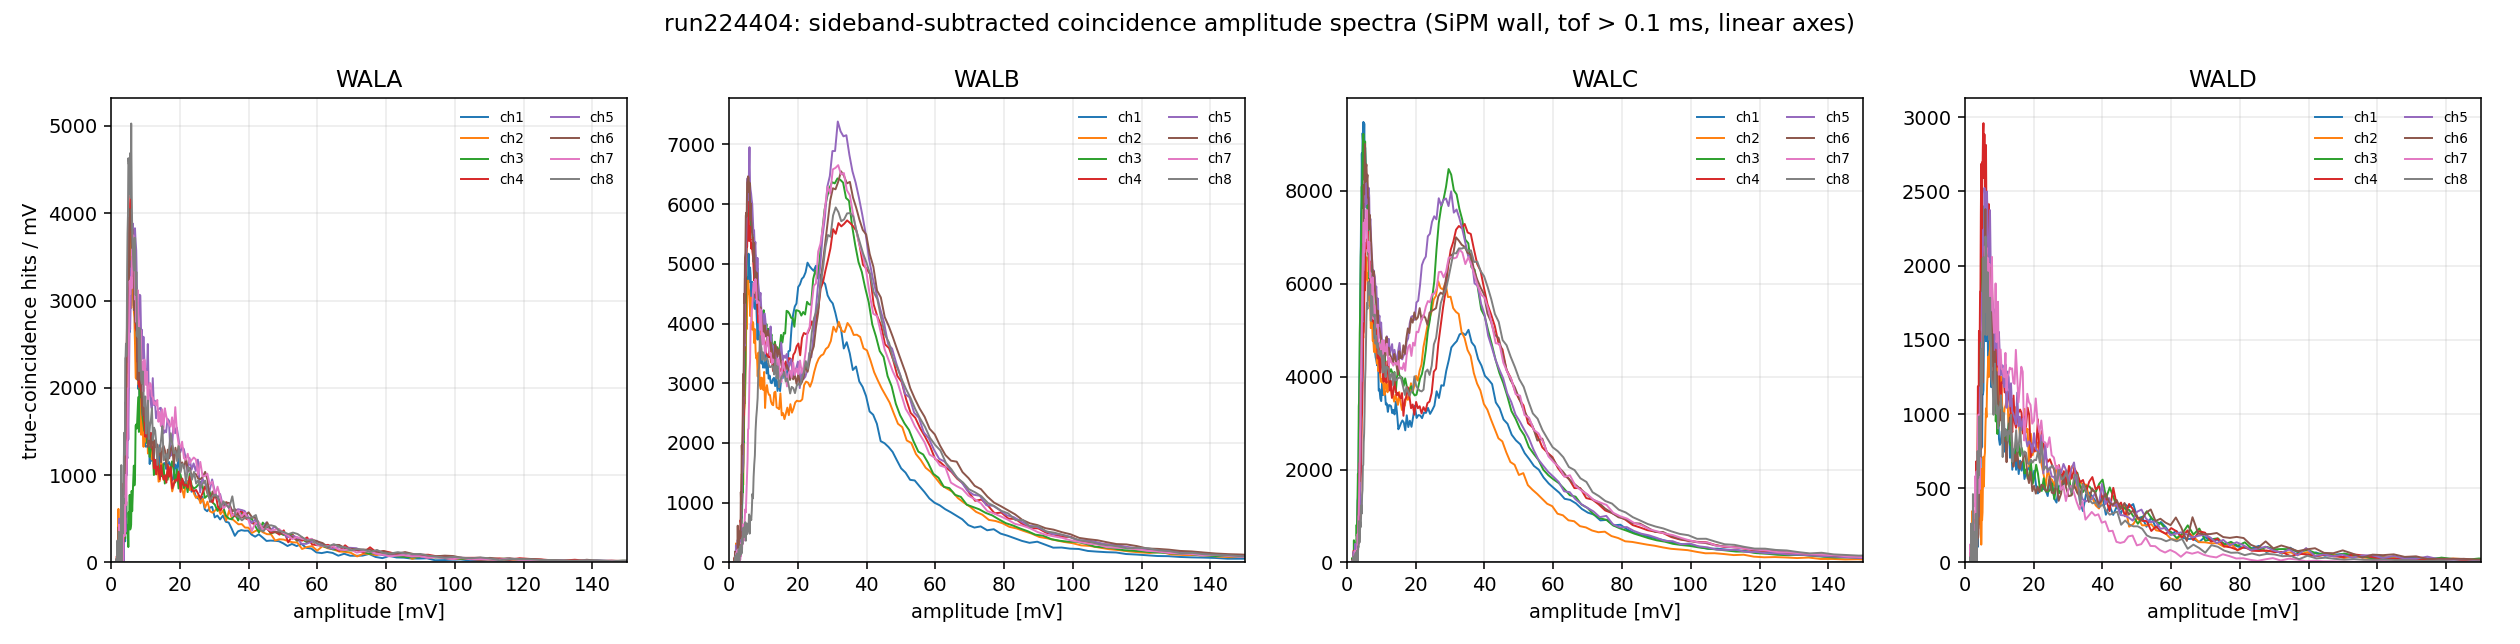
\includegraphics[width=\textwidth]{06_07_geometry_mip/mip_wall_spectra_linear.png}
\column{.45\textwidth}
\begin{itemize}
\item A/D: 6--8$\times$ fewer true coincidences; coincident spectrum just traces
      the inclusive shape --- no MIP bump.
\item Hypotheses: (i) plastic response misses MIPs; (ii) wall SiPM gain low;
      (iii) geometry, absorption, or flux composition.
\item Inclusive plastic medians agree within $\pm$30\% across all 8 PMTs
      (PSSD1 highest) $\Rightarrow$ large plastic-gain deficit unlikely.
\item Wall-only top--bottom check (backup): SiPM response healthy on all four
      arms; but same-scintillator coincidence cannot distinguish through-going
      tracks from local deposits (e.g.\ $\gamma$/Compton), so the cause
      remains open.
\item Follow-ups: pre-flash cosmic sample (guaranteed through-going muons),
      LIQ readout, plastic HV scan.
\end{itemize}
\end{columns}
\end{frame}

\begin{frame}{Plastic PMT relative gains \& HV suggestions}
\centering\small
\begin{tabular}{lrrrrr}
\toprule
PMT & HV [V] & med$_\mathrm{inc}$ [mV] & rel.\ gain & $V$(equalize) & $V$($2\times$) \\
\midrule
PSSA1 (AL) & 1325 & 10.4 & 0.74 & 1384 & 1528 \\
PSSA2 (AR) & 1275 & 13.2 & 0.93 & 1288 & 1422 \\
PSSB1 (BL) & 1325 & 13.1 & 0.93 & 1339 & 1478 \\
PSSB2 (BR) & 1300 & 14.9 & 1.05 & 1290 & 1425 \\
PSSC1 (CL) & 1300 & 14.5 & 1.03 & 1295 & 1429 \\
PSSC2 (CR) & 1300 & 15.3 & 1.08 & 1285 & 1419 \\
PSSD1 (DL) & 1300 & 17.8 & 1.26 & 1258 & 1389 \\
PSSD2 (DR) & 1300 & 14.9 & 1.06 & 1290 & 1424 \\
\bottomrule
\end{tabular}\\[1ex]
{\footnotesize $G\propto V^{7}$ assumed --- request a 2-point HV scan to calibrate.}
\end{frame}

\begin{frame}{Raw vs coincidence-selected plastic spectra (per PMT)}
\centering
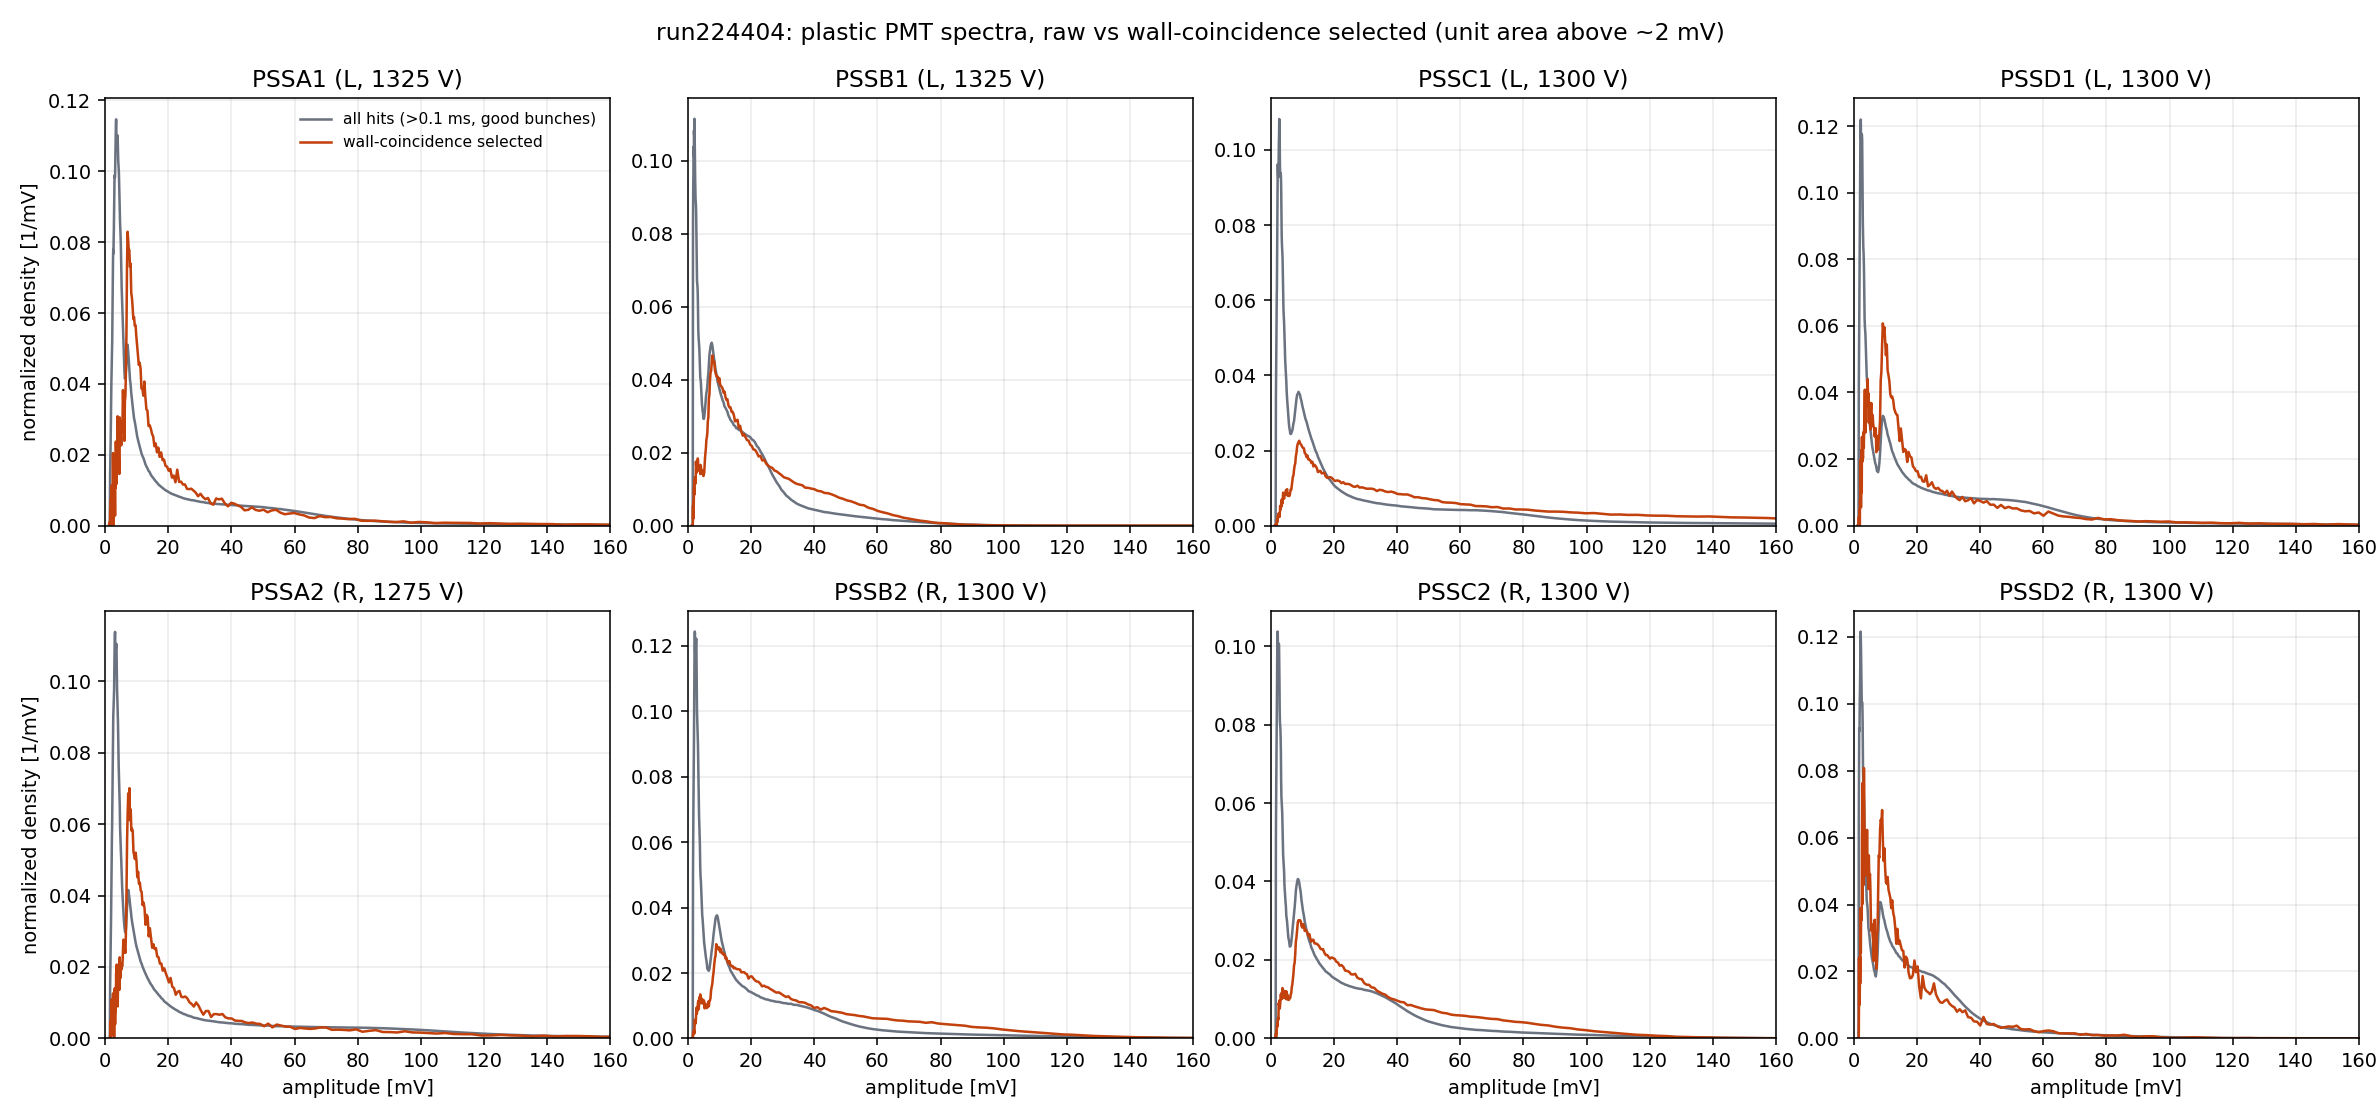
\includegraphics[width=.95\textwidth]{10_pmt_gain/pmt_raw_vs_coinc.png}
\end{frame}

\begin{frame}{What we want to enable later today: LIQ readout}
\centering
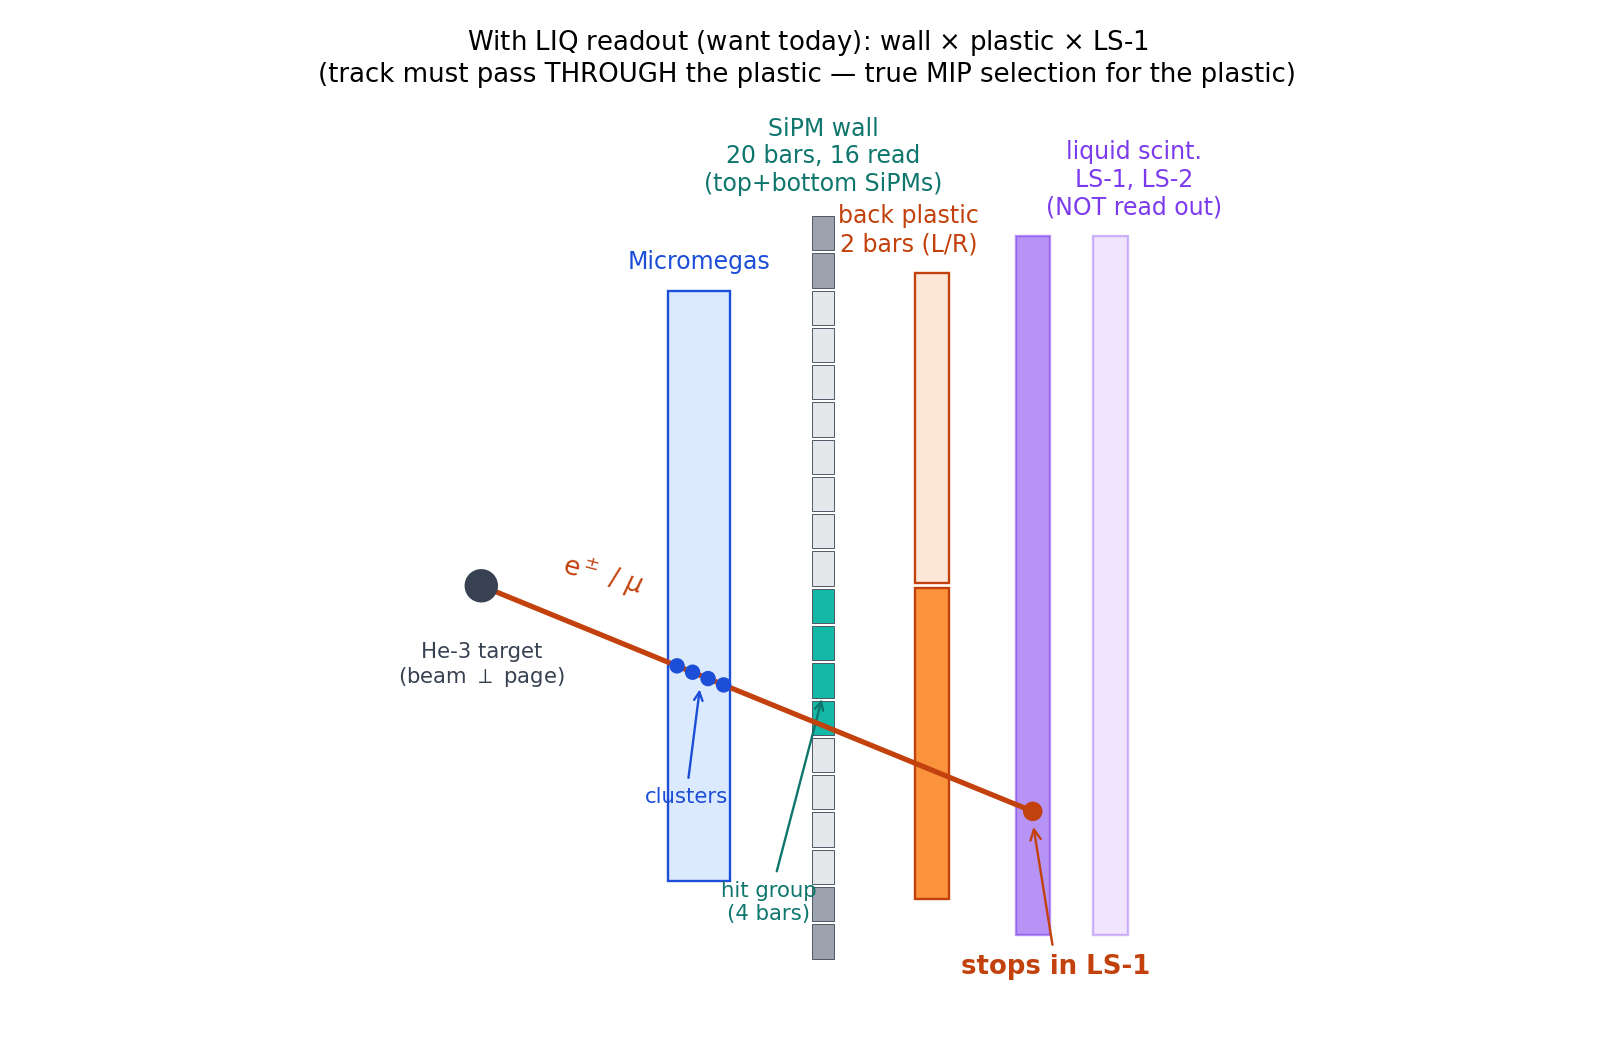
\includegraphics[height=.82\textheight]{11_diagrams/concept_wall_plastic_liq.png}
\end{frame}

\begin{frame}{Requests}
\begin{enumerate}
\item \textbf{Read out the liquid scintillators} (behind the plastic):
      wall+LIQ coincidence requires passage \emph{through} the plastic
      $\Rightarrow$ true plastic MIP calibration. Only LIQA/LIQD cabled, no data.
\item Plastic HV scan (2 points) $\rightarrow$ apply gain equalization.
\item Cabling confirmations: top/bottom card assignment; which 4 of 20 wall
      bars unread; physical arm positions A--D.
\item DAQ follow-up on the SiPM-wall outage (bunches 643--2212).
\end{enumerate}
\end{frame}

\begin{frame}{Backup: wall-only top--bottom coincidences}
\centering
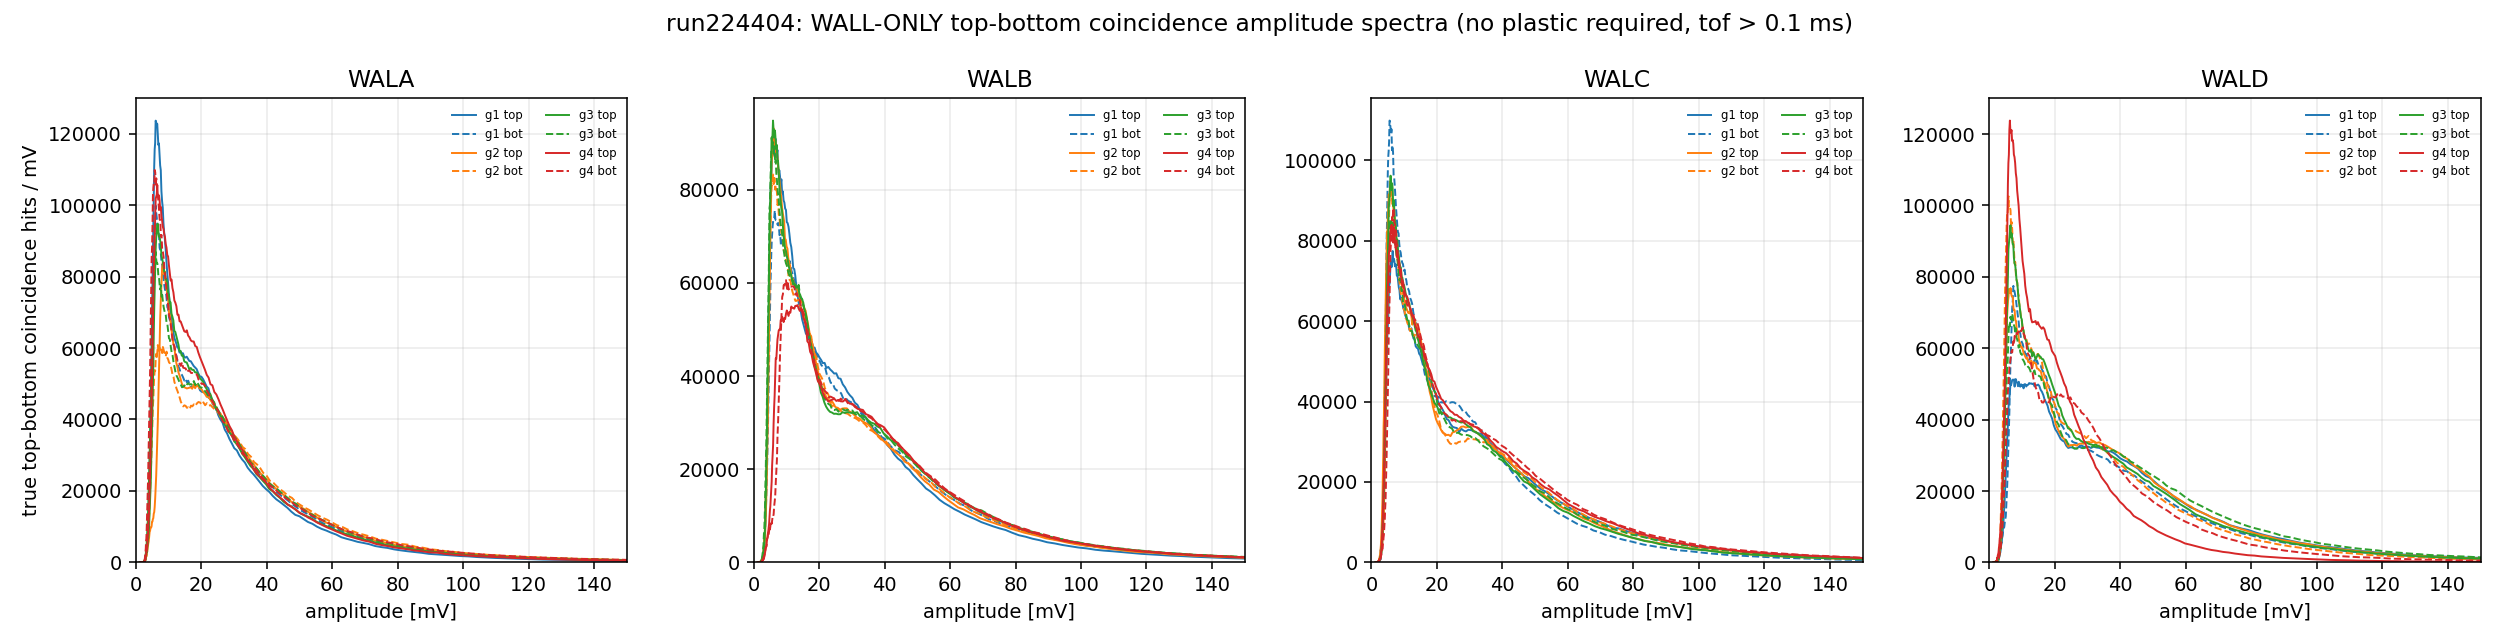
\includegraphics[width=.9\textwidth]{06_07_geometry_mip/wall_topbot_spectra.png}
\begin{itemize}\footnotesize
\item Top \& bottom SiPMs read the \emph{same} 4-bar group: any real deposit
      (through-going MIP, stopping e$^\pm$, or a $\gamma$ Compton-scattering in
      the bars) lights both ends in tight coincidence --- removes noise, not
      physics backgrounds.
\item Shows: SiPM response/gain healthy on all four arms (MIP-scale bump
      25--40 mV everywhere); an amplitude landmark for all 32 channels.
\item Cannot show: whether particles traverse onward to the back plastic ---
      the A/D deficit remains unattributed (plastic response, absorption
      between wall and plastic, or flux composition).
\end{itemize}
\end{frame}

\begin{frame}{Backup: window scan \& purity}
\centering
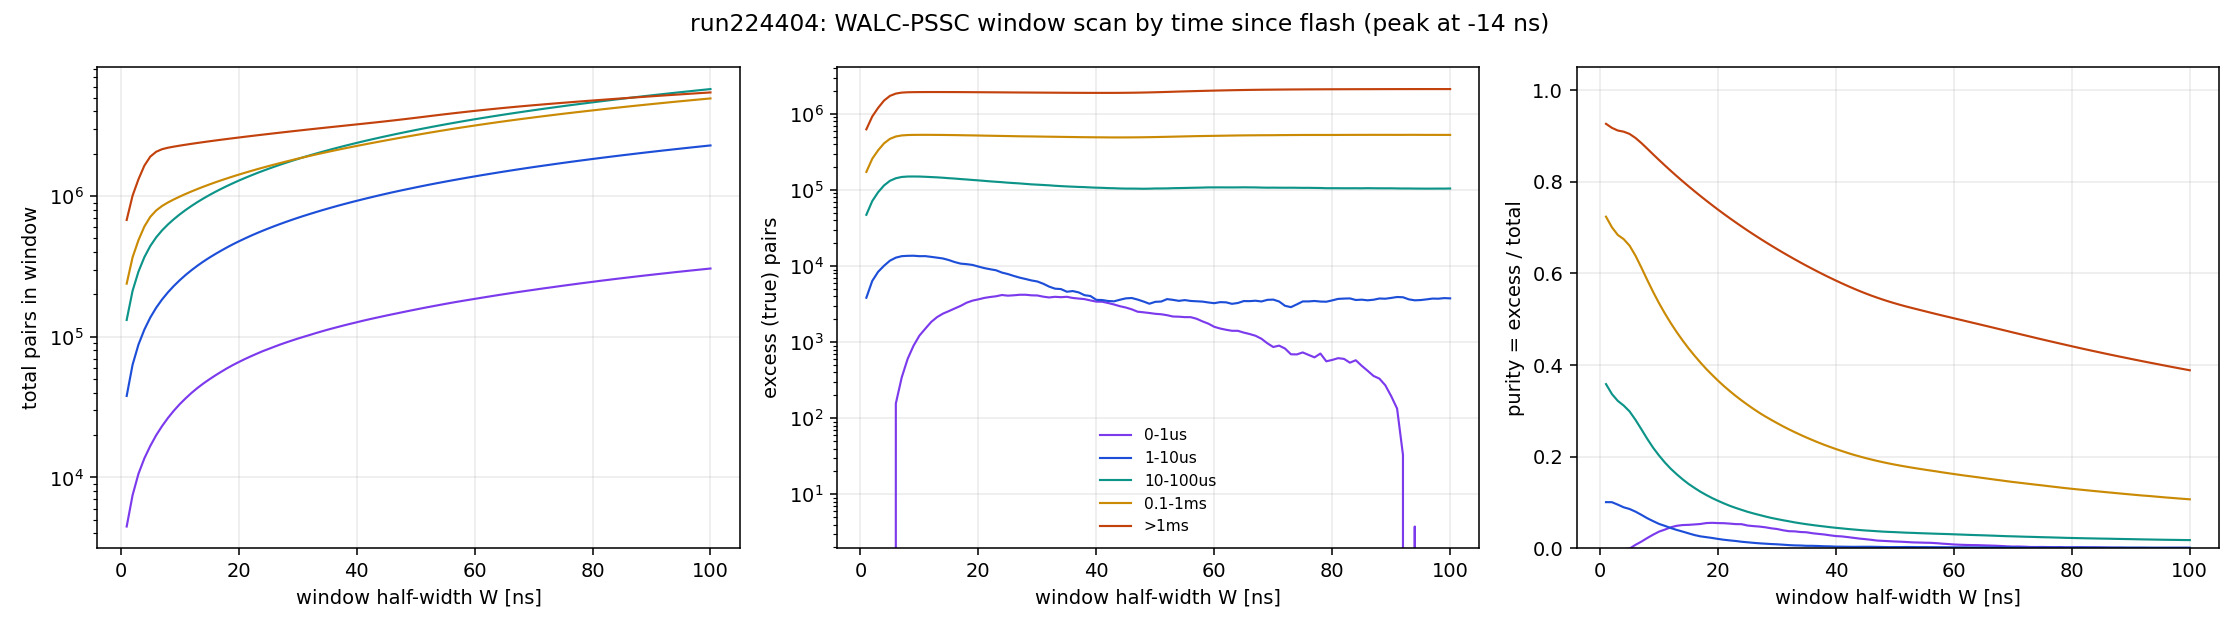
\includegraphics[width=.9\textwidth]{02_coincidence/window_scan_regions_WALC_PSSC.png}
\end{frame}

\begin{frame}{Backup: full QA}
\centering
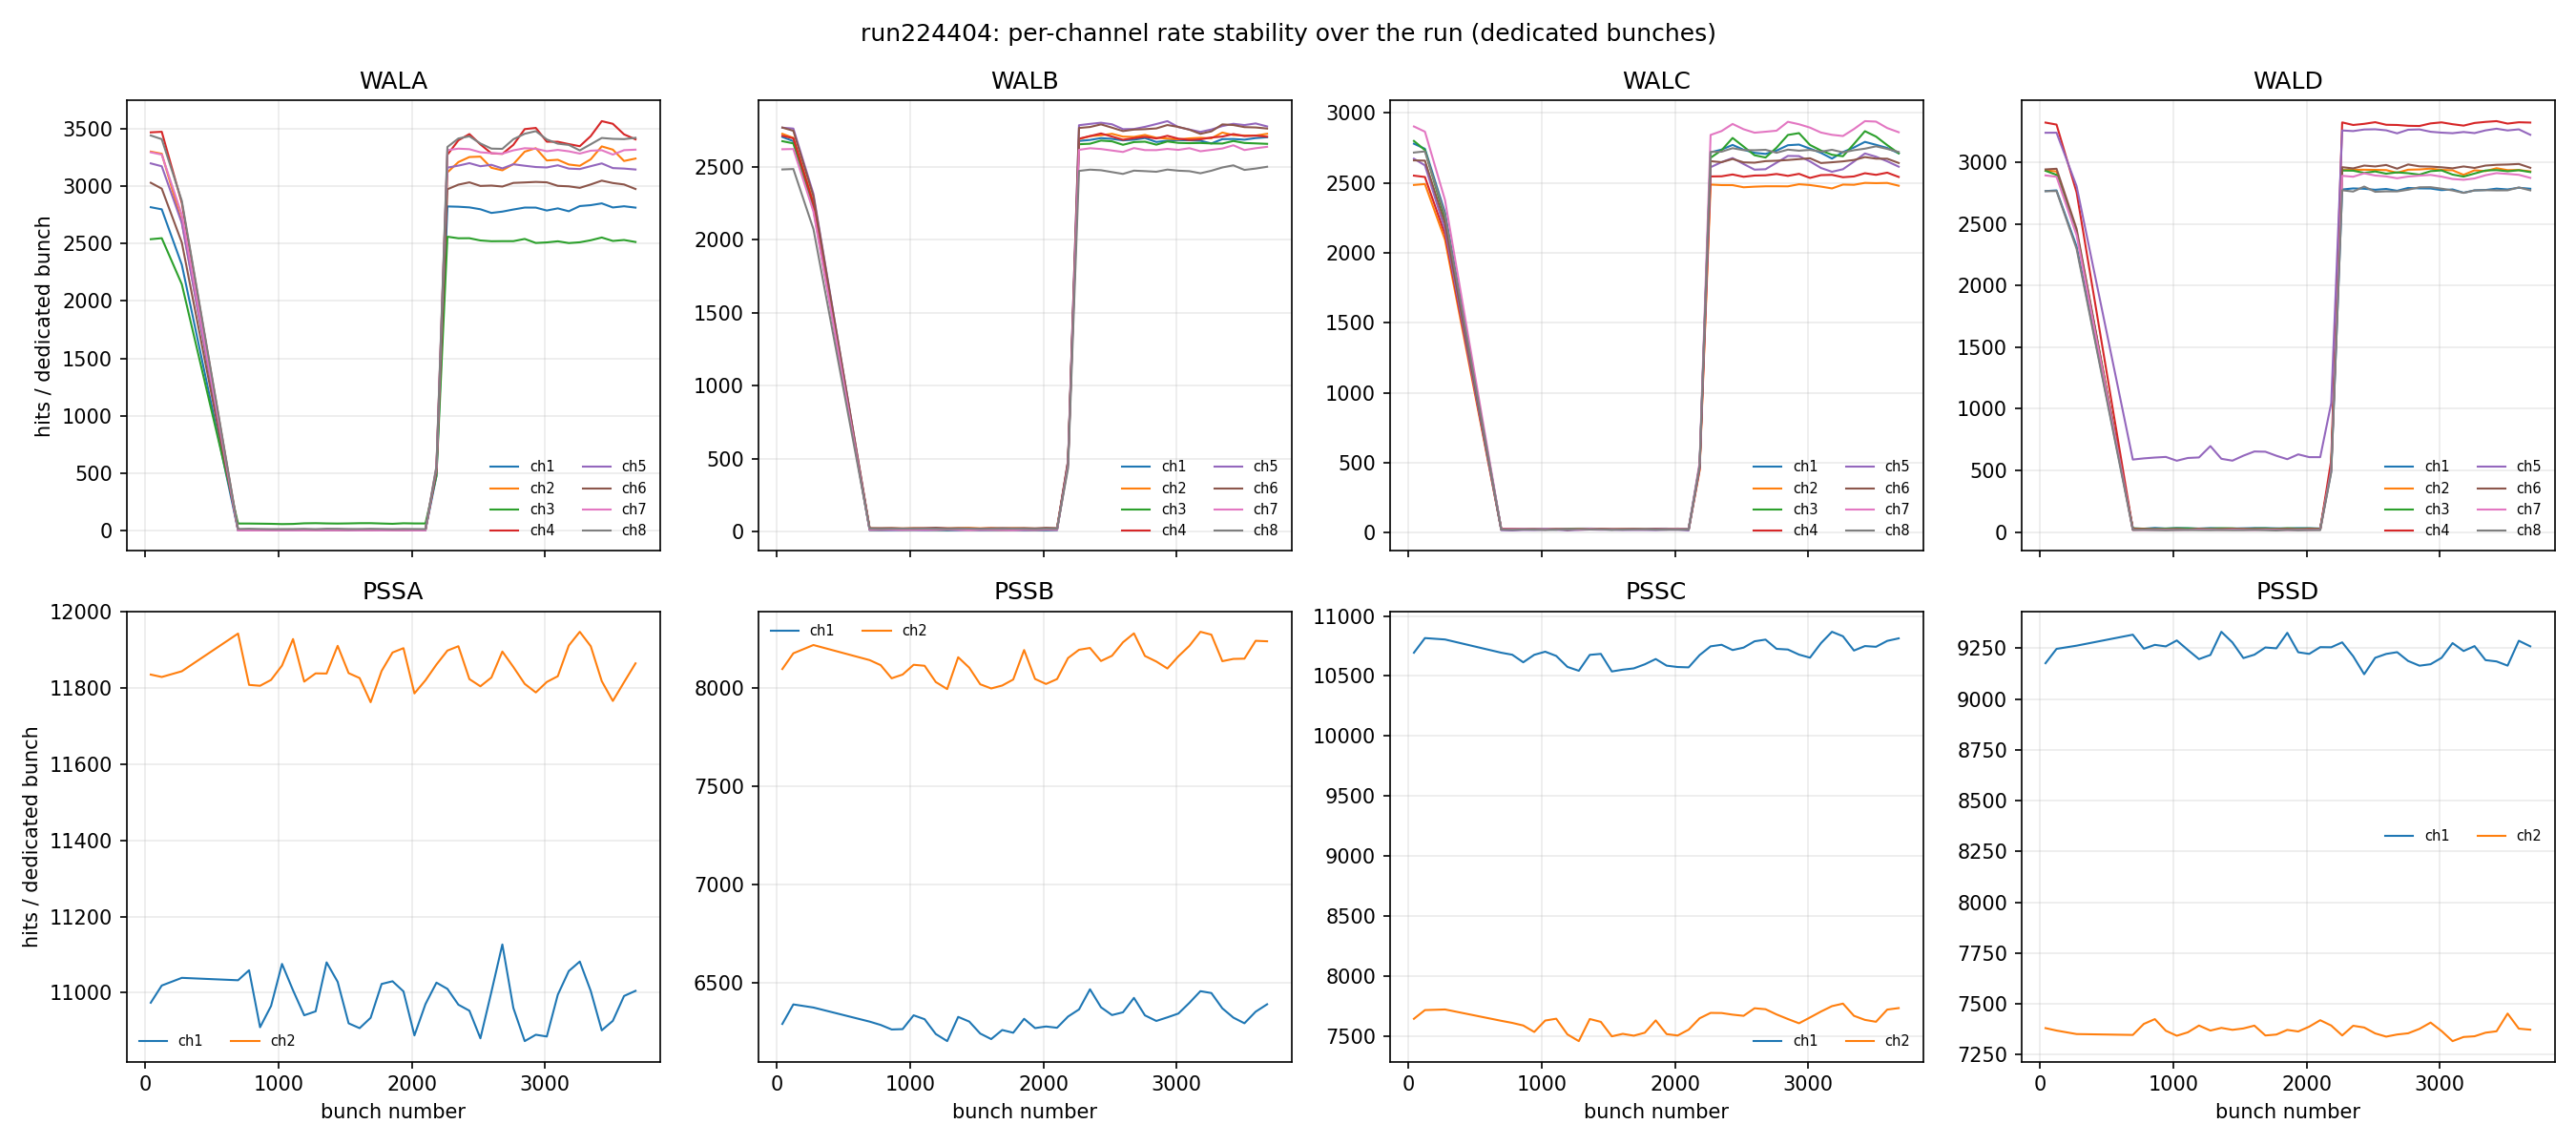
\includegraphics[width=.85\textwidth]{01_signal_qa/rate_stability.png}
\end{frame}

\end{document}
